\begin{center}
	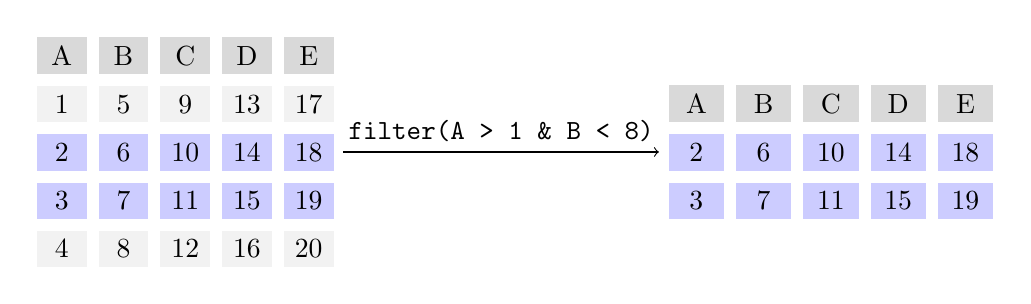
\begin{tikzpicture}
		\matrix (a) [
			column sep = 1 ex, row sep = 1 ex, shape = rectangle, minimum height = 1 em, minimum width = 1.8 em,
			row 1/.style = {nodes = {fill = gray!30}},
			row 2/.style = {nodes = {fill = gray!10}},
			row 3/.style = {nodes = {fill = blue!20}},
			row 4/.style = {nodes = {fill = blue!20}},
			row 5/.style = {nodes = {fill = gray!10}}
		] {
        			\node {A}; &
        			\node {B}; &
        			\node {C}; &
        			\node {D}; &
        			\node {E}; \\
			\node {1}; &
			\node {5}; &
			\node {9}; &
			\node {13}; &
			\node {17}; \\
			\node {2}; &
			\node {6}; &
			\node {10}; &
			\node {14}; &
			\node {18}; \\
			\node {3}; &
			\node {7}; &
			\node {11}; &
			\node {15}; &
			\node {19}; \\
			\node {4}; &
			\node {8}; &
			\node {12}; &
			\node {16}; &
			\node {20}; \\
		};
		\begin{scope} [xshift = 8.2 cm]
            		\matrix (b) [
            			column sep = 1 ex, row sep = 1 ex, shape = rectangle, minimum height = 1 em, minimum width = 2 em,
            			row 1/.style = {nodes = {fill = gray!30}},
            			row 2/.style = {nodes = {fill = blue!20}},
            			row 3/.style = {nodes = {fill = blue!20}}
            		] {
                			\node {A}; &
                			\node {B}; &
                			\node {C}; &
                			\node {D}; &
                			\node {E}; \\
            			\node {2}; &
            			\node {6}; &
            			\node {10}; &
            			\node {14}; &
            			\node {18}; \\
            			\node {3}; &
            			\node {7}; &
            			\node {11}; &
            			\node {15}; &
            			\node {19}; \\
            		};
		\end{scope}
		\draw[->] (a) -- (b) node[midway, above] {\tt filter($\texttt{A > 1~\&~B < 8}$)};
	\end{tikzpicture}
\end{center}
\begin{center}
	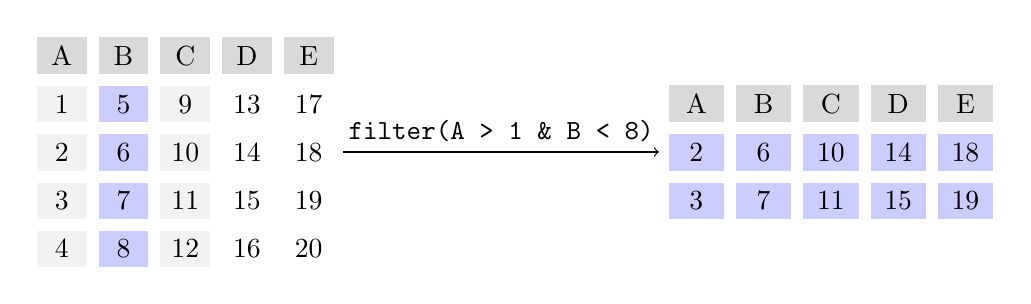
\begin{tikzpicture}
		\matrix (a) [
			column sep = 1 ex, row sep = 1 ex, shape = rectangle, minimum height = 1 em, minimum width = 1.8 em,
			column 1/.style = {nodes = {fill = gray!10}},
			column 2/.style = {nodes = {fill = blue!20}},
			column 3/.style = {nodes = {fill = gray!10}},
			row 1/.style = {nodes = {fill = gray!30}},
		] {
        			\node {A}; &
        			\node {B}; &
        			\node {C}; &
        			\node {D}; &
        			\node {E}; \\
			\node {1}; &
			\node {5}; &
			\node {9}; &
			\node {13}; &
			\node {17}; \\
			\node {2}; &
			\node {6}; &
			\node {10}; &
			\node {14}; &
			\node {18}; \\
			\node {3}; &
			\node {7}; &
			\node {11}; &
			\node {15}; &
			\node {19}; \\
			\node {4}; &
			\node {8}; &
			\node {12}; &
			\node {16}; &
			\node {20}; \\
		};
		\begin{scope} [xshift = 8.2 cm]
            		\matrix (b) [
            			column sep = 1 ex, row sep = 1 ex, shape = rectangle, minimum height = 1 em, minimum width = 2 em,
            			row 1/.style = {nodes = {fill = gray!30}},
            			row 2/.style = {nodes = {fill = blue!20}},
            			row 3/.style = {nodes = {fill = blue!20}}
            		] {
                			\node {A}; &
                			\node {B}; &
                			\node {C}; &
                			\node {D}; &
                			\node {E}; \\
            			\node {2}; &
            			\node {6}; &
            			\node {10}; &
            			\node {14}; &
            			\node {18}; \\
            			\node {3}; &
            			\node {7}; &
            			\node {11}; &
            			\node {15}; &
            			\node {19}; \\
            		};
		\end{scope}
		\draw[->] (a) -- (b) node[midway, above] {\tt filter($\texttt{A > 1~\&~B < 8}$)};
	\end{tikzpicture}
\end{center}
 
